\chapter{Bildverarbeitung und Umsetzung}
\label{cha:verarbeitungumsetzung}

\section{Kalibrierung}
\label{sec:kalibrierung}

F"ur eine Messung, bei der der Fehler minimiert werden soll, ist das Kalibrieren der Kameras unumg"anglich. Bei der Kamerakalibrierung werden mehrere Parameter bestimmt. Diese beeinflussen die Kameras und die Weltkoordinaten:

\begin{description}
	\item[Intrinsische Parameter]
	Sind kameraspezifische Parameter. Hier bei handelt es sich um Hardwareeigenschaften der Kamera.\newline
	Das Berechnen der intrinsischen Werte ist essentiell für das Eliminieren der Verzerrung der Linse. Dadurch kann eine 3D-Punkteberechnung stattfinden.
	
	\item[Extrinsische Parameter]
	Beschreiben die Kameraposition und Rotation in Weltkoordinaten.
\end{description}

\noindent Da es ich bei dem System um ein Stereokamera-System handelt, ist die Kalibrierung von diesem etwas komplizierter.\newline
Zuerst m"ussen die Kameras gesondert kalibriert werden. Dies wird mit der Funktion \textit{calibrateCamera} von OpenCV durchgef"uhrt. F"ur die Kalibrierung wird ein Schachbrett-Muster verwendet. Wichtig ist, dass bei der Kalibrierung beide Kameras dasselbe Bild verwenden. F"ur die Erkennung des Schachbretts wird die OpenCV-Funktion \textit{findChessboardCorners} verwendet. Diese liefert die Objekt- und Bild-Punkte der Aufnahme. Bei den Objekt-Punkten handelt es sich um die 3D-Punkte des Bildes, bei den Bild-Punkten um die 2D-Punkte\cite{OcvD}.
\noindent F"ur eine m"oglichst genaue Kalibrierung werden 50 Bilder verwendet. Anhand dieser Bilder wird jede Kamera mittels \textit{calibrateCamera} kalibriert. Anschlie"send wird das Ergebnis dieser Kalibrierungen an die OpenCV-Funktion \textit{stereoCalibrate} "ubergeben.




\begin{figure}[H]
	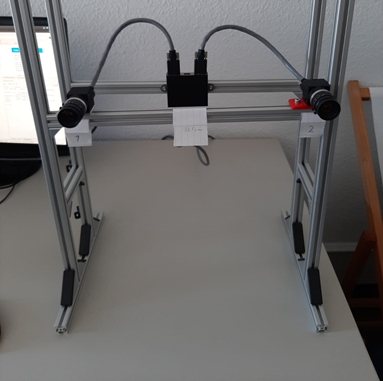
\includegraphics[scale=0.3]{bilder/camerasystem}
	\caption[Kamera-System]{Kamera-System}
\end{figure}
